\section{Sprint 2}

\subsection{Sprint planning}

	\subsubsection{Expected results}
  From this sprint, we expect to have a working local storage on the phone. This will provide persistence of observations in the phone. In addition, the document will be ready for the pre-delivery 6th of October.
	
	\subsubsection{Duration}
	Start of Sprint 2 is September 26th, and it will last until October 9th (weeks 39 and 40). Customer meeting is on October 11th, just after the completion of whole sprint. Advisor meetings are on September 27th and October 4th.

\subsection{Requirements}

\begin{description}
	\item[F10] Autocomplete should be able to load data based on species category
	\item[F2] User must be able to add more information to a species observation
	\item[F6] User must be able to view observations stored on the device
	\item[F7] User must be able to edit a stored observation on the device
\end{description}

\subsection{Implementation}

A species in the observation can now have more information added to it via the 'Extended Information' page.
A click on the details button is caught by JQuery, the id of the species is found by finding the parents of the button in the DOM, where a div contains the id.
The activeExtended attribute in Observation is set so that species and the application transitions to the Extended Information page, values from the species object is read and filled in with JQuery.
When transitioning back to the Observation page, all informations are saved to the object again and the row of the edited species is updated on the Observation page.

The user may now view stored observations, a button for this has been made functional on the main page.
\paragraph{ObservationList.js} populates a list of saved observations.
The user can select an observation, identified by which species category it is related to and when it was created as well as it's id.
When an observation is selected, two global variables related to the id of the observation and it's speciesgroup are set and the user is redirected to the Observation page.
The observation is read from storage and loaded into the DOM, editable in the same way as when first created in order to create a simple and easily recongnizable interface.

This uses the same code as when a new observation is created, however when a new one is created the global variables are unset and a new observation object is created instead by main.js.

	\subsubsection{Auto-complete}

	Auto-complete has been extended to read files based on species category.
	Initially each category was included in a separate file, but this caused some
	performance issues due to the large amount of data (browser freeze while reading
	files). To circumvent this issue, the team decided to split the categories into
	multiple files, keeping one folder per category and one file per prefix see.

	To achieve this, following conventions / specifications will be used:

	\begin{itemize}
		\item Auto-Complete data is rooted in the directory WEBROOT/data/autocomplete
		\item Each species category will get a sub-folder under the auto-complete
		root. This will be named after the category id (an integer).
		\item Each category directory should contain one index.js file that
		keeps an overview of all the prefix-files for the category.
		\item Files in the category directory are named by the following rules:
			\begin{itemize}
				\item a.json contains only entries prefixed by a
				\item a\_b.json contains entries prefixed by a or b (can be
				extended with more entries)
				\item a-z.json contains entries prefixed by a, b, c, ..., or z
				\item a\_c-e\_q\_t contains entries prefixed by a, c, d, e, q, or t
			\end{itemize}
	\end{itemize}

	\subsubsection{Storage}
	\label{sec:storage}

	Storing observations locally on the phone is achieved using the PhoneGap
	local storage API, which is based on the W3C Web SQL database specification
	and W3C Web Storage API specification. In short, it uses the SQLite database
	management system to store data.

	The database consists of three tables:
	\begin{itemize}
		\item Observations, which contains the observation id, location, create date, and the group of the species (bird, mammal, fish, etc. For identifying the type of observation)
		\item Species, which contains the actual data of the observation, type of species, age, sex, etc.
		\item Pictures, which contains an uri to the images attached to each species (The image itself is stored somewhere else on the phone, depending on the device/camera app)
	\end{itemize}
	
	\begin{figure}[htb]
		\centering
		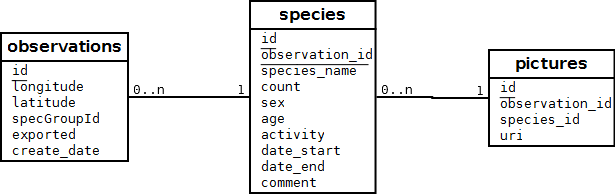
\includegraphics[width=0.8\textwidth]{sprints/db_diagram.png}
		\caption{Diagram showing the database tables and their relations}
		\label{fig:dbdiagram}	
	\end{figure}
	
	The reason the database is split like this is to allow each observation to
	contain many species, and allow each species to contain many pictures. See
	figure \ref{fig:dbdiagram} for details. The two latter tables have the
	primary key(s) of the preceding table as foreign key(s).
	
	The storage is implemented in the ObservationDao.js file, which contains
	methods to initialize the database, as well as various methods to store and
	retrieve entries for observations, species and pictures.
				
\subsection{Testing}

We focused primarily on unit testing and informal testing in a "sandbox"
environment. Informal testing consisted of visual inspection of the user
interface and unstructured functional testing (i.e. functional testing that we
did not document). The informal testing gave some ideas as to how we could
develop and document our functional tests later in the project, it was also
helpful in verifying that functionality in the frameworks worked as expected.




\begin{table}[htb]
	\label{sprint2:unit-testing-table}
	\centering
    \resizebox{1.0\textwidth}{!}{
    \begin{tabular}{|l|p{5cm}|l|l|}
		\hline
		Module & Test description & Number of assertions & Result \\
		\hline \hline
		AutocompleteDao & should set categoryRoot to directory above index.js when loaded & 1 & PASS \\ \hline
		AutocompleteDao & should fail gracefully if loading file by category fails & 1 & PASS \\ \hline
		AutocompleteDao & should be able to load file based on prefix & 6 & PASS \\ \hline
		AutocompleteDao & should be able to determine if term can be completed with current prefix & 5 & PASS \\ \hline
		Autocomplete & should return 0 suggestions on no matches & 2 & PASS \\ \hline
		Autocomplete & should return 3 ordered suggestions on exactly 3 matches & 5 & PASS \\ \hline
		Autocomplete & should return 6 ordered suggestions on exactly 6 matches & 16 & PASS \\ \hline
		Autocomplete & should return 6 ordered suggestions on more than 6 matches & 8 & PASS \\ \hline
		Autocomplete & should be able to activate autocomplete for input element & 2 & PASS \\ \hline
    \end{tabular}}
  \caption{Excerpt from unit testing}
\end{table}
By "sandbox" environment we refert to testing on a PC, in addition to using a
debug-section of the app that will be removed before project completion on
mobile devices.
By re-running the unit tests from sprint 1 we had efficient regression testing.
This was very helpful in the process of expanding functionality. We have
developed a complete set of unit tests for the auto-complete and storage
functionality. Table \ref{sprint2:unit-testing-table} contains an excerpt from
the unit testing.

In conclusion, we used unit testing for functionality that has well defined
input- and output parameters. Other functionality, like the user interface were
tested by visual inspection and informal functional testing.

\subsection{Customer feedback}
The customer was happy with our current progress. As this was a big sprint for
us, we couldn't fully complete all our items in the sprint backlog. The customer
stressed that we start thinking about how to do the export functionality for the
next sprint.

\subsection{Evaluation}
The implementaion of the main part of the application went as expected, with the
main focus on creating a good storage system and improving the autocomplete from
the previous sprint. The creation of the storage system also made it possible to
create sections required in the specifications such as viewing and editing
observations.

Auto-complete now works with satisfactory speed, even on the slower devices. Splitting the files allowed even the largest files to load sufficiently fast. However, it is not yet using the correct data. This will be rectified in a later sprint.

After this sprint the storage module allows for correctly and reliably storing and retrieving observations and their attached species. PhoneGap's storage API made it a bit simpler than writing to file, which was our initial approach to the problem.
